\section{Visualization of the graphs}
Graphs are fascinating structures, visualizing them can give us a more deep understanding of their proprieties. To do that we need to make some sacrifices. We are dealing with millions of nodes, displaying them all would be impossibile, especially on a web page as I did. \s

\nd For each case we need to find a small (in the order of 1000) subset of nodes $S \subset V$ that we want to display. It's important to take into consideration, as far as we can, nodes that are "important" in the graph \s

\nd All this section is implemented in python using the library \texttt{pyvis}. The goal of this library is to build a python based approach to constructing and visualizing network graphs in the same space. A pyvis network can be customized on a per node or per edge basis. Nodes can be given colors, sizes, labels, and other metadata. Each graph can be interacted with, allowing the dragging, hovering, and selection of nodes and edges. Each graph's layout algorithm can be tweaked as well to allow experimentation with rendering of larger graphs. It is designed as a wrapper around the popular Javascript \texttt{visJS} library

\subsection{Actors Graph}
For the actors graph we choose the subset $S$ as the actors with at least 100 movies made in their carrier. We can immediately deduct that this subset will be characterized by actors and actresses of a certain age. But as we have seen, having an high number of movies made it's a good estimator for the closeness centrality. It's important to keep in mind that the graph will only show the relations nodes in this subset. This means that even if an actor has 100 movies made in his carrier, in this graph may have just a few relations. We can see this graph as collaboration network between the most popular actors and actresses. \s

\nd An interactive version can be found at this web page. It will take a few seconds to render, it's better to use a computer and not a smartphone. \s

\textsc{Interactive version}: \url{https://lukefleed.xyz/imdb-graph.html}

\begin{center}
    \s \nd \qrcode{https://lukefleed.xyz/imdb-graph.html}
\end{center}

\begin{figure}[H] \label{imdb-a-network}
    \centering
    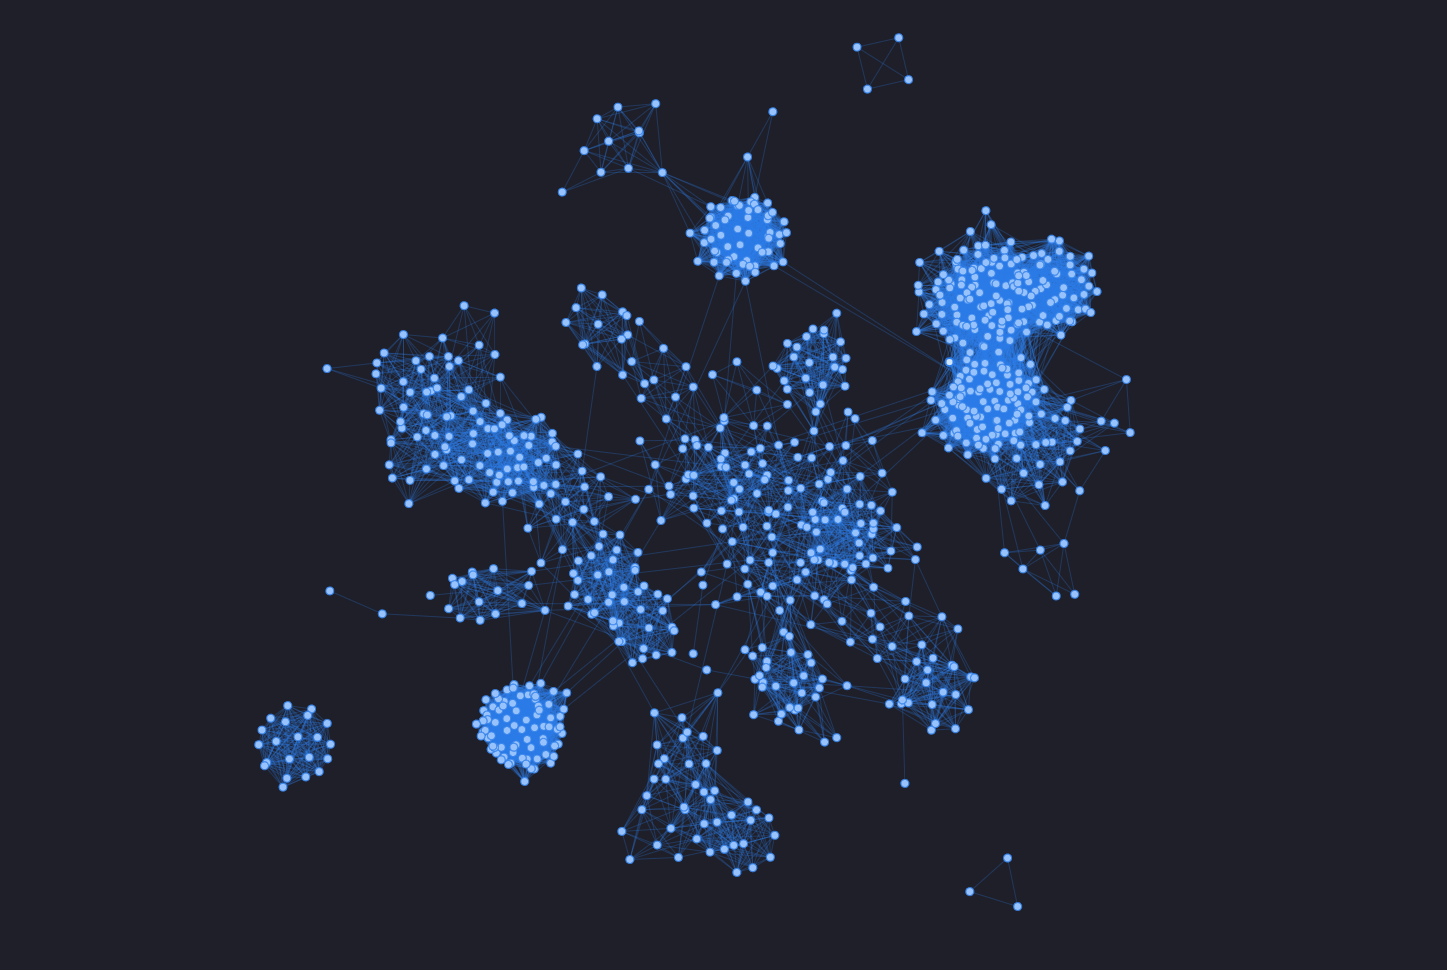
\includegraphics[width=13cm]{Screenshot.png}
    \caption{\emph{The collaboration network of the actors and actresses with more that an 100 movies on the IMDb network}}
\end{figure}

The results obtained is extremely interesting. We can clearly see how this graph it's characterized by different (and some times isolated) communities. The nodes in them are all actors and actresses of the same nationality. There are some very big clusters as the \emph{Bollywood}'s one that are almost isolated. Due to cultural and linguistic differences those actors never collaborated with anyone outside their country. \s

A visual analysis of this graph can reflects some of the proprieties that we saw during the analysis of the results. Let's take the biggest cluster, the Bollywood one. Even if it's very dense and the nodes have a lot of links, none of them ever appeared in out top-k results during the testing. This happens due to the proprieties of closeness centrality, the one that we are taking into consideration. It can be seen as the ability of a node to transport information efficiently into the graph. But the Bollywood's nodes are efficient in transporting information only in their communities. \s

A simple and heuristic way to see this phenomena is by grabbing in the interactive graph a node with an higher centrality and dragging him around. We'll see that it will drag with him every community. If we repeat the same action with a Bollywood node, it will only move the nodes of his community, leaving almost un-moved all the other nodes
